% Combined "stacked embedding spaces" figure: the same archive is embedded into
% three metric spaces, drawn as a stack of identical isometric planes, each
% measured by its own operation (covering radius / nearest-noun).
% Designed so an animation can flip which plane is on top.
% Assets (*_iso.png, cap_thumb_*.png, _recall_meta.tex, _semantic_meta.tex) built
% by tools/build_metric_fig_assets.py --only iso recall.
% Compile: pdflatex metric_spaces_stack.tex
\documentclass[border=8pt, varwidth=false]{standalone}
% Shared TikZ styling for the eval-metric pipeline figures, matching the look of
% paper/system_fig/system_overview.tex. \input after \documentclass{standalone}.
\usepackage{tikz}
\usetikzlibrary{positioning,shapes.geometric,arrows.meta,calc,fit,backgrounds,fadings}
\usepackage{graphicx}
\usepackage{amsmath,amssymb}
\usepackage{xcolor}
\usepackage[T1]{fontenc}

\tikzset{
  >=Stealth,
  box/.style       = {draw, rounded corners=2pt, align=center,
                      inner sep=4pt, line width=0.6pt, fill=white},
  vlmbox/.style    = {box, fill=blue!5,    draw=blue!55!black},
  embbox/.style    = {box, fill=violet!7,  draw=violet!60!black},
  databox/.style   = {box, fill=black!3,   draw=black!45},
  scorebox/.style  = {box, fill=orange!12, draw=orange!75!black, line width=0.9pt},
  img/.style       = {draw=black!45, line width=0.4pt, inner sep=0, outer sep=0},
  pipe/.style      = {->, line width=0.7pt, draw=black!75},
  feed/.style      = {->, line width=0.9pt, draw=orange!75!black},
  frame/.style     = {draw=black!45, line width=0.5pt, rounded corners=4pt,
                      inner sep=10pt},
  colTitle/.style  = {font=\bfseries, anchor=south west},
}


\IfFileExists{_recall_meta.tex}{% auto-generated by tools/build_metric_fig_assets.py
\def\recallCells{0/cockatoo/0.151, 1/teapot/0.146, 2/parrot/0.145, 3/eye/0.143, 4/kettle/0.141, 5/owl/0.140}
\def\recallScore{0.087}
\def\recallNumNouns{1{,}823}
}{%
  \def\recallNumNouns{1{,}823}}
\IfFileExists{_semantic_meta.tex}{% auto-generated by tools/build_metric_fig_assets.py
\def\captionCells{0/{A black and white line drawing of the silhouette of a sports car.}, 1/{A black and white drawing of a Stormtrooper helmet.}, 2/{A minimalist black and white line drawing of a cat looking up.}}
\def\visualScore{0.606}
\def\semanticScore{0.686}
}{%
  \def\captionCells{0/{A black and white line drawing of the silhouette of a sports car.},
    1/{A black and white drawing of a Stormtrooper helmet.},
    2/{A minimalist black and white line drawing of a cat looking up.}}}

% per-plane accent colours (match the baked PNG overlays)
\definecolor{visAcc}{HTML}{C01515}
\definecolor{semAcc}{HTML}{B8860B}
\definecolor{recAcc}{HTML}{7A52C0}

% throughline edge colours: one for the image domain (archive images and their
% embeddings), one for the text domain (VLM captions, THINGS nouns and their
% text embeddings).  The VLM captioner is the single crossover where the image
% domain (blue) turns into the text domain (orange).
\definecolor{imgEdge}{HTML}{1F6FB2}
\definecolor{txtEdge}{HTML}{C8721A}

\begin{document}
\begin{tikzpicture}[font=\normalsize, x=1cm, y=1cm,
  plabel/.style={anchor=west, align=left, inner sep=2pt},
  % right-hand metric header: sized (in the exported SVG) to match the blog's
  % HTML triptych headers (CMU bold, ~22px at desktop widths).  Blog-only figure.
  % \fontseries{b} = Computer Modern Bold (cmb), NOT the default \bfseries cmbx
  % (Bold Extended); this matches the blog's cmb10.ttf HTML triptych headers.
  mhead/.style={anchor=west, align=left, inner sep=2pt,
                font=\fontsize{18}{21}\fontseries{b}\selectfont},
  % plain-language gloss under each header ("what does this metric ask?")
  subq/.style={anchor=north west, align=left, inner sep=2pt, text width=4.3cm,
               text=black, font=\large},
  chip/.style={scorebox, anchor=north west, align=left, font=\scriptsize},
  % orange feed line WITHOUT an arrowhead, for intermediate / merging segments
  % (arrowheads live only on the final segment that lands on a node/plane)
  feedline/.style={line width=0.9pt, draw=orange!75!black},
  % modality-coloured edges: image domain (blue) vs text domain (orange).
  % *feed = lands on a node/plane (arrowhead); *line = intermediate (no head).
  imgfeed/.style={->, line width=0.9pt, draw=imgEdge},
  imgline/.style={line width=0.9pt, draw=imgEdge},
  txtfeed/.style={->, line width=0.9pt, draw=txtEdge},
  txtline/.style={line width=0.9pt, draw=txtEdge}]

% ---- geometry ----
\def\PW{8.2cm}      % plane image width (all three PNGs are identical)
\def\Cx{21}         % shared plane centre x
% row order top->bottom: Image (visual), Image&Text (recall), Text (semantic).
\def\Vy{0}          % image      plane north y  (top)
\def\Ry{-3.4}       % image+text plane north y  (middle)  (even 3.4 spacing)
\def\Sy{-6.8}       % text       plane north y  (bottom)
\def\Lx{25.7}       % right-hand label column x
% the planes are identical in height, so equal anchor spacing gives equal
% vertical whitespace between them.  We no longer hardcode the plane mid-heights
% (which drift whenever the *_iso.png aspect ratios change); instead the left-hand
% feed sources and right-hand labels are anchored directly to each plane's .west
% (see (vW)/(rW)/(sW) below), so every feed arrow is self-correctingly horizontal.

% ===================== SOURCE: ARCHIVE =====================
\node[frame, minimum width=4.2cm, minimum height=4.2cm, anchor=north west]
  (arch) at (0,-2.4) {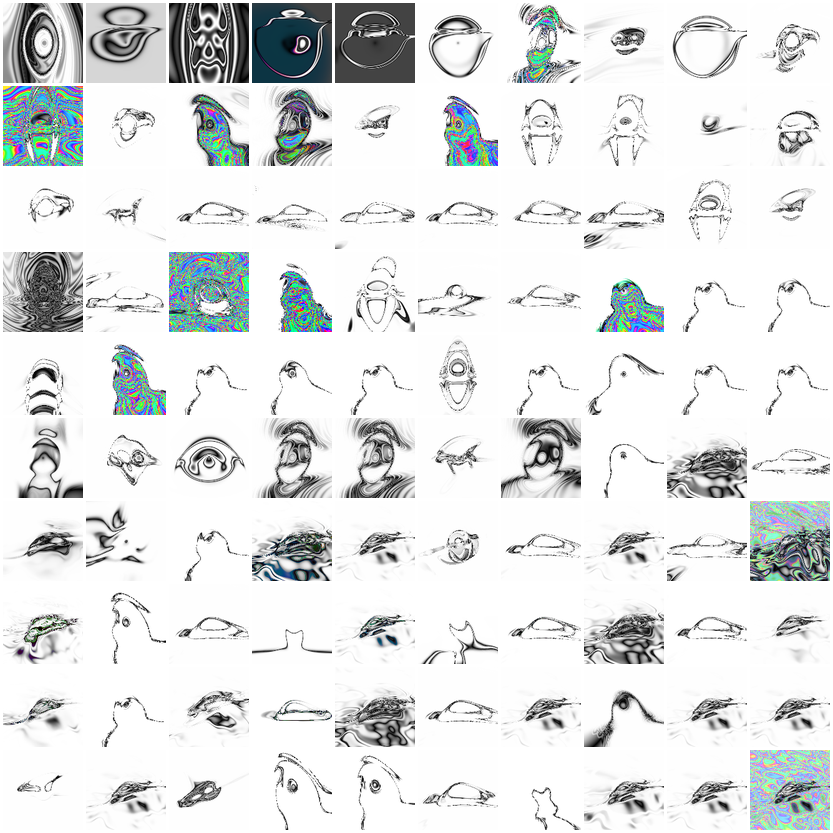
\includegraphics[width=3.6cm]{archive_grid.png}};
\node[colTitle] at (arch.north west) {Archive};

% branch point: the archive feeds all three throughlines.  Its y is tied to the
% archive box's true .east (keeping x=5.0) so the feeder line is dead flat
% regardless of the framed box's exact height.
\coordinate (br) at (5.0,0 |- arch.east);
% archive emits images (blue) into both the image-embedding branch and the
% VLM captioner branch; the captioner is where it turns into text (orange).
\draw[imgline] (arch.east) -- (br);

% ===================== STACKED ISOMETRIC PLANES =====================
\node[anchor=north] (rP) at (\Cx,\Ry) {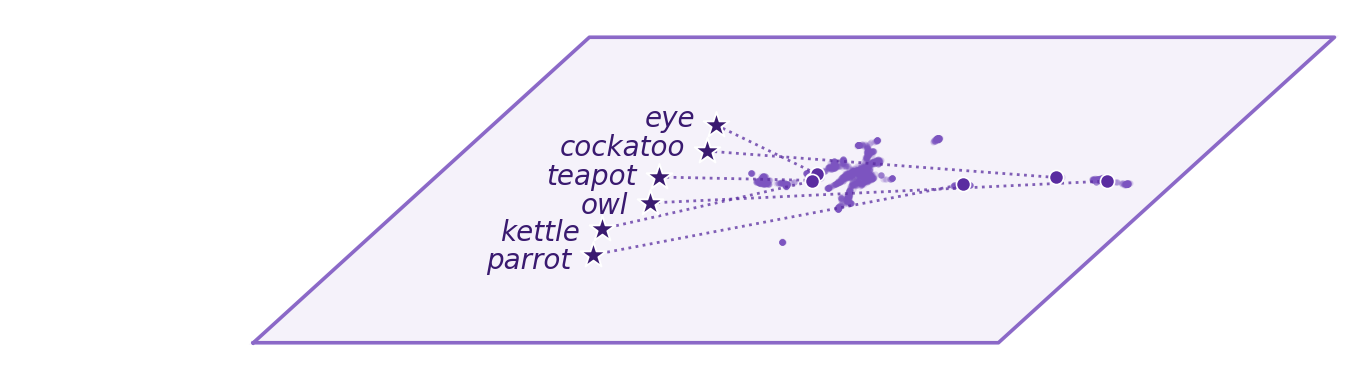
\includegraphics[width=\PW]{recall_iso.png}};
\node[anchor=north] (sP) at (\Cx,\Sy) {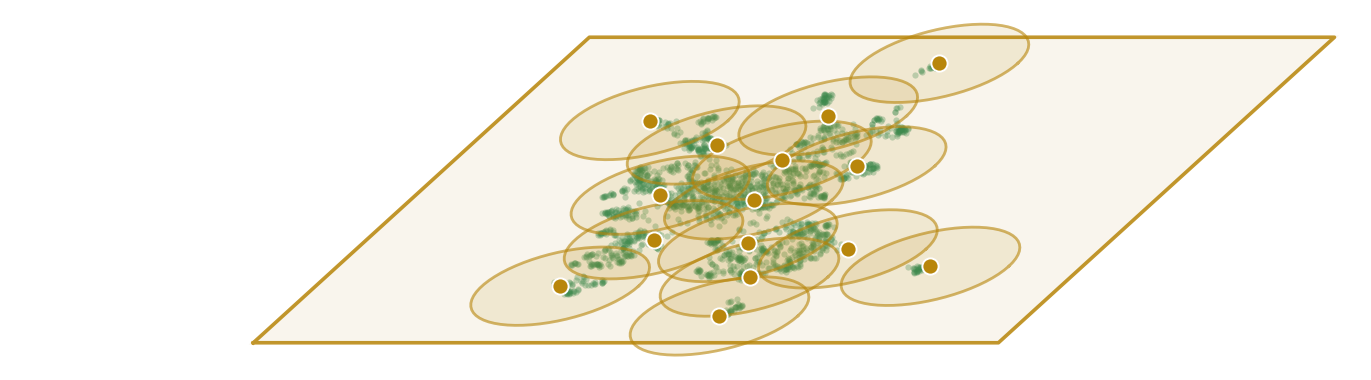
\includegraphics[width=\PW]{semantic_iso.png}};
\node[anchor=north] (vP) at (\Cx,\Vy) {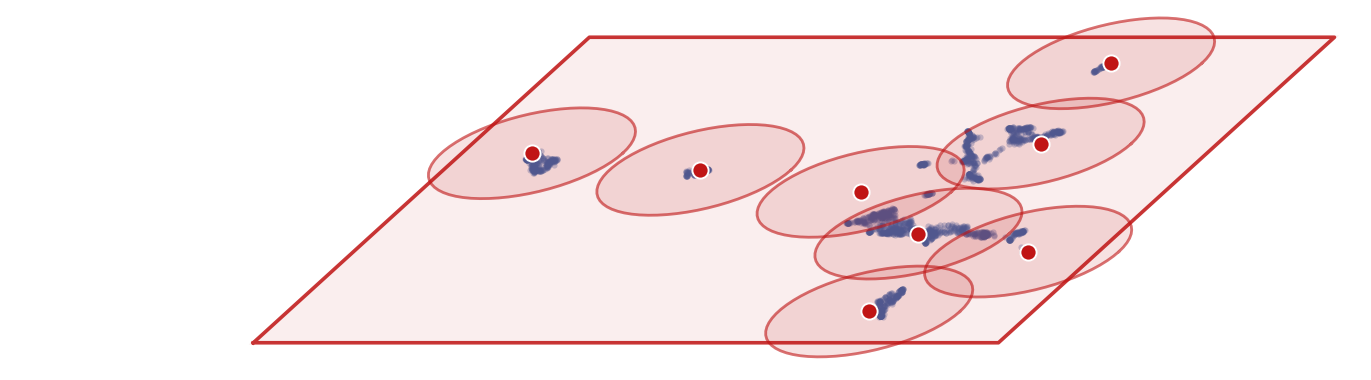
\includegraphics[width=\PW]{visual_iso.png}};

% Self-correcting plane-centre coordinates: each plane's true .west anchor sits
% at its rendered vertical midpoint REGARDLESS of the PNG's aspect ratio.  Every
% left-hand feed source and right-hand label hangs off these, so all three feed
% arrows are guaranteed horizontal and land at the plane's left-edge midpoint.
\coordinate (vW) at (vP.west);   % top    (image / Visual)
\coordinate (rW) at (rP.west);   % middle (image+text / Recall)
\coordinate (sW) at (sP.west);   % bottom (text / Semantic)
% the joint Image&Text plane receives two SEPARATE arrows -- the reused image
% embedding (blue) lands on its upper-left, the noun text embedding (orange) on
% its lower-left -- so the two modalities stay visually distinct on the plane.
\coordinate (rjImg) at ([xshift=1.6cm, yshift=0.45cm]rP.west);
% rjTxt is tied to the text-embedding box's height (set below) so its inbound
% arrow is flat; defined as a coordinate later, once tnN exists.

% title naming each embedding space (Archive-style label), above the slab
\node[colTitle] at ([xshift=3.0cm, yshift=0.04cm]vP.north west) {Image Embeddings};
\node[colTitle] at ([xshift=3.0cm, yshift=0.04cm]sP.north west) {Text Embeddings};
\node[colTitle] at ([xshift=3.0cm, yshift=0.04cm]rP.north west) {Image \& Text Embeddings};

% ---- per-throughline transforms (each line shows its real operations) ----
% Shared image embedding: the archive is embedded once here and the SAME
% embedding feeds BOTH the Visual plane and the Recall plane (no re-embedding).
% imN's y is tied to vP's .west via |- (keeping its original x): node-centre y
% == vP.west y, so imN.east y == plane-entry y and the feed is dead flat.
\node[embbox, anchor=west, text width=2.1cm] (imN) at (6.6,0 |- vW)
  {image\\ embedding};
\draw[imgfeed] (br) |- (imN.west);
% the image embedding is reused: one straight, perfectly horizontal landing on
% the Visual plane (top), and one smooth curve down to the joint Recall plane
% (middle) where it lands on its own (no merge with the noun text embedding).
\draw[imgfeed] (imN.east) -- ([xshift=1.6cm]vP.west);
% flipped-S: leaves the image-embedding box horizontally, swings down, and
% arrives horizontally on the joint plane (both tangents flat -> S, not a swoop)
\draw[imgfeed] (imN.east) .. controls +(3.2,0) and +(-3.2,0) .. (rjImg);

% Semantic: image -> VLM caption -> caption examples -> text embedding.
% The Captions panel is defined first so the flanking VLM-caption and text-embed
% boxes can be centred on it -> the (capN->cap) and (cap->tEmb) arrows are flat.
% Only the first two captions are shown, with a vertical ellipsis below to signal
% "and more" -- keeps the panel short so its title doesn't crowd the nouns row.
\node[frame, anchor=north west, minimum width=5.0cm, minimum height=3.6cm]
  (cap) at (8.5,-6.14) {};
\node[colTitle, align=left] at (cap.north west) {Captions};
\coordinate (cgo) at ([xshift=0.85cm, yshift=-0.95cm]cap.north west);
\foreach \ic/\cp in \captionCells {%
  \ifnum\ic<2\relax
  \node[img] (ct-\ic) at ([yshift={-\ic*1.35cm}]cgo)
    {\includegraphics[width=0.85cm]{cap_thumb_\ic.png}};
  \node[anchor=west, text width=3.0cm, font=\scriptsize, align=left, inner sep=2pt]
    at ([xshift=0.5cm]ct-\ic.east) {``\cp''};
  \fi
}
% vertical ellipsis under the thumbnail column -> "and more captions"
\node[font=\large] at ([yshift=-0.75cm]ct-1) {$\vdots$};
% VLM-caption and text-embed boxes vertically centred on the Captions panel, so
% both arrows that touch the panel are perfectly horizontal.
\node[vlmbox, anchor=west, text width=1.85cm] (capN) at (5.4,0 |- cap.west)
  {VLM caption};
\node[embbox, anchor=west, text width=1.7cm] (tEmb) at (15.6,0 |- cap.east)
  {text embed};
% archive image enters the captioner (still image domain -> blue); everything
% downstream of the VLM caption is text (orange).
\draw[imgfeed] (br) |- (capN.west);
\draw[txtfeed] (capN.east) -- (cap.west);
\draw[txtfeed] (cap.east) -- (tEmb.west);
% flat landing on the Semantic plane, raised to the text-embed box's height
\draw[txtfeed] (tEmb.east) -- ([xshift=1.6cm]sP.west |- tEmb);

% Recall: the THINGS noun set embedded into the SAME SigLIP2 text-image space,
% joined with the reused archive image embedding -> joint text-image plane.
% tnN's y tied to the Recall plane's .west via |- (keeping its x) so the
% (tnN.east) feed is level.
\node[embbox, anchor=west, text width=1.9cm] (tnN) at (10.5,0 |- rW)
  {text\\ embedding};
% THINGS box sits to the left; its bottom is aligned with the text-embedding
% box's bottom (anchor south west tied to tnN's .south y).
\node[databox, anchor=south west, text width=3.3cm, align=center]
  (nouns) at (5.8,0 |- tnN.south) {%
  \textbf{Nouns}\\[2pt]
  {\itshape\scriptsize duck, teapot, eye, car,\\ owl, dolphin, parrot, \dots}};
% lower-left landing on the joint plane, level with the text-embedding box so the
% arrow is flat; separate from the image embedding's blue arrow above.
\coordinate (rjTxt) at ([xshift=1.6cm]rP.west |- tnN);
% flat arrow into the text-embedding box: leave the THINGS box's right edge at
% the text-embedding box's height (lower than the box's mid) so the line is level.
\draw[txtfeed] (nouns.east |- tnN.west) -- (tnN.west);
% flat landing on the joint Image&Text plane, raised to the text-embedding box's
% height, separate from the image embedding's blue arrow above.
\draw[txtfeed] (tnN.east) -- (rjTxt);

% ===================== PER-PLANE: METRIC NAME + SPACE + QUANTITY =====================
% (metric names live here on the right; no absolute numbers -- only meaningful
%  comparatively across runs)
% Each label stacks: metric name (plane-accent) -> operation chip (orange box)
% -> plain-language question.  The name's baseline is aligned to each plane's
% north edge, so it sits level with the "... Embeddings" title on the left
% (same anchor + yshift as those colTitle nodes above the planes).
\coordinate (vLt) at (\Lx,0 |- vP.north);
\coordinate (rLt) at (\Lx,0 |- rP.north);
\coordinate (sLt) at (\Lx,0 |- sP.north);

\node[mhead, text=visAcc, anchor=south west] (vt) at ([yshift=0.04cm]vLt) {Visual Coverage};
\node[chip] (vc) at ([yshift=-0.13cm]vt.south west) {$k$-covering radius};
\node[subq] at ([yshift=-0.11cm]vc.south west) {``How different do these images look?''};

\node[mhead, text=recAcc, anchor=south west] (rt) at ([yshift=0.04cm]rLt) {Semantic Recall};
\node[chip] (rc) at ([yshift=-0.13cm]rt.south west) {mean distance of nearest\\ image over all nouns};
\node[subq] at ([yshift=-0.11cm]rc.south west) {``How much do they look like things?''};

\node[mhead, text=semAcc, anchor=south west] (st) at ([yshift=0.04cm]sLt) {Semantic Coverage};
\node[chip] (sc) at ([yshift=-0.13cm]st.south west) {$k$-covering radius};
\node[subq] at ([yshift=-0.11cm]sc.south west) {``How many things do they look like?''};

\end{tikzpicture}
\end{document}
